%Config
\documentclass[12pt,twoside]{article}
\usepackage[spanish,es-tabla]{babel}
\usepackage[a4paper]{geometry}

\usepackage{graphicx}               % Para incluir imágenes
\usepackage{amsmath}                % Para el manejo de matemáticas
\usepackage{url}
\usepackage{float}

\title{Autómata Celular Elemental y la regla 30}
\author{Erick Jesse Angeles López}


% Definir un comando para palabras clave
\newcommand{\keywords}[1]{%
	\begin{center}
		\textbf{Palabras clave:} #1
	\end{center}
}

\renewcommand{\baselinestretch}{1}
\setcounter{page}{1}
\setlength{\textheight}{21.6cm}
\setlength{\textwidth}{14cm}
\setlength{\oddsidemargin}{1cm}
\setlength{\evensidemargin}{1cm}
\pagestyle{myheadings}
\thispagestyle{empty}
\markboth{\small{Ángeles López Erick Jesse}}{\small{Automata celular elemental y la regla 30}}
\date{}

\begin{document}
	
	\begin{center}
		
		% Contenido izquierdo - Imagen
		\begin{minipage}{0.17\textwidth}
			\centering
			
\includegraphics[width=0.7\textwidth]{img/ipn_logo.jpg} % Ajusta esta línea
		\end{minipage}
		\begin{minipage}{.55\textwidth}
			\centering
			{\Large Instituto Politécnico Nacional}\\
			{\Large Escuela Superior de Cómputo}
		\end{minipage}
		\begin{minipage}{0.17\textwidth}
			\centering
			
\includegraphics[width=0.9\textwidth]{img/escom_logo} % Ajusta esta línea
		\end{minipage}			
	\end{center}
	
	
	\centerline{\bf Ingeniería en Inteligencia Artificial, Algoritmos Bioinspirados}
	
	\centerline{\bf  Sem: 2025-1, 5BM1, Fecha: FECHA}
	
	\centerline{}
	
	%\centerline{}
	
	
	\begin{center}
		\Large{\textsc{Autómata Celular Elemental y la regla 30}} 
	\end{center}
	\centerline{}
	\centerline{\bf {\textit{Presenta}}}
	\centerline{\bf {Angeles López Erick Jesse\footnote{eangelesl1700@alumno.ipn.mx}}}
	\centerline{}
	\centerline{}
	\centerline{\bf {Disponible en:}}
	\centerline{\text{\url{GITHUB}}}
	
	
	
	
	\newtheorem{Theorem}{\quad Theorem}[section]
	
	\newtheorem{Definition}[Theorem]{\quad Definition}
	
	\newtheorem{Corollary}[Theorem]{\quad Corollary}
	
	\newtheorem{Lemma}[Theorem]{\quad Lemma}
	
	\newtheorem{Example}[Theorem]{\quad Example}
	
	\bigskip
	
	\bigskip
	
	\begin{abstract} 
		
	\end{abstract}
	
	\keywords{}
	
	\clearpage
	
	\tableofcontents
	\clearpage
		
	\section{Introducción}
	
	Los autómatas celulares (AC, de ahora en adelante, por su traducción al inglés: ``Cellular Automaton'') fueron concebidos por John Von Neumann en 1948 mientras buscaba diseñar un sistema capaz de auto-replicarse, es decir, un robot con la capacidad de construir otro robot. Las limitaciones físicas lo llevaron a seguir el consejo de Stanislaw Ulam, quien le sugirió diseñar un modelo matemático discreto con esta capacidad de auto-reproducción.
	
	Los AC se definen como un conjunto de celdas o células que adquieren diferentes valores según la interacción que se produce entre ellas. Matemáticamente, un AC se describe mediante una 4-tupla:
	
	\begin{equation*} CA = \{L, S, N, f\} \end{equation*}
	
	Donde: 
	\begin{itemize} \item $\boldsymbol{L}$: Espacio dimensional. Define la dimensionalidad de una rejilla de células agrupadas. Este espacio es (teóricamente) infinito.

		\item $\boldsymbol{S}$: Conjunto finito de estados que puede adquirir cada célula dentro del espacio asignado.
		
		\item $\boldsymbol{N}$: Define las posiciones relativas de cada célula que formarán parte de la vecindad. El comportamiento de cada célula depende de su vecindad.
		
		\item $\boldsymbol{f : S^{[N]} \rightarrow S}$: Función de transición. Determina el próximo valor de cada célula en función de los valores de las células vecinas. Esta actualización se realiza de manera simultánea en cada periodo de tiempo discreto.
	\end{itemize}
	
	Estos sistemas permiten simular diversos fenómenos, como el comportamiento de ecosistemas en biología, la detección de incendios en bosques o el tráfico vehicular en diferentes ciudades.
	
	Dos de los AC más conocidos son el Juego de la Vida, propuesto por John Conway, y el Autómata Celular Elemental, desarrollado por Stephen Wolfram.
	
	El Juego de la Vida de Conway consiste en un conjunto de células en un espacio bidimensional, un conjunto de estados binarios, una vecindad de Moore (las 8 células circundantes) y una función que define la vida o muerte de cada célula con base en la población viva de su vecindad.
	
	Por otro lado, el Autómata Celular Elemental es una colección de autómatas que comparten un espacio unidimensional, un conjunto de estados binarios y una vecindad de radio uno (la célula en cuestión y sus dos células vecinas más cercanas). Dichos autómatas se diferencian únicamente en la función de transición, que puede adoptar hasta 256 ``reglas'' o configuraciones diferentes.
	
	Una de estas reglas, conocida y patentada por Wolfram como Regla 30, presenta un comportamiento errático y aparentemente aleatorio. Si se inicia con una única célula viva, esta se expande en ambas direcciones con cada iteración, siendo capaz de llenar todo el espacio. Sin embargo, el comportamiento de la célula inicial no parece seguir un patrón discernible.
	
	Por ello, en este reporte se busca \dots
	
	\clearpage
	\section{Marco Teórico}
	
	\subsection{Autómata Celular Elemental}
	
	El autómata celular elemental (ECA, de ahora en adelante, por su traducción al inglés: ``Elementary Cellular Automaton'') se caracteriza por su simplificación de los autómatas celulares y su comportamiento divergente.
	
	Sus características principales son:
	
	\begin{itemize}
		\item Una dimensión: $L = 1$. Es decir, las células están agrupadas en una línea infinita de forma consecutiva.
		
		\item Dos estados posibles por célula: $S = \{0, 1\}$.  
		
		\item Vecindad local: La vecindad de cada célula se define por sí misma y sus dos vecinas más cercanas, también llamado radio 1. La posición relativa está dada por $N = \{-1, 0, 1\}$.  
		
		\item Funciones de transición: Dado que la vecindad está conformada por tres células y cada célula puede adquirir dos valores, existen $|S|^{|N|} = 2^3 = 8$ combinaciones posibles de vecindad. Además, como cada combinación puede tener dos reglas de producción, es decir, generar un 0 o un 1, existen $|S|^{|S|^{|N|}} = 2^{2^3} = 2^8 = 256$ autómatas celulares diferentes.  
		
	\end{itemize}
	
	A cada combinación de vecindad se le puede asociar un número binario determinado por el valor de cada célula. Dado que existen 8 combinaciones, cada ECA se puede representar mediante un número binario de 8 dígitos, lo que, traducido a base decimal, adquiere un valor (y el nombre) entre 0 y 255.
	
	En la figura \ref{img:eca1}, se muestra la configuración de la regla 210, que equivale a $210_{10} = 11010010_2$. Las casillas negras representan los unos, y las blancas, los ceros.
	
	\begin{figure}[H]
		\centering
		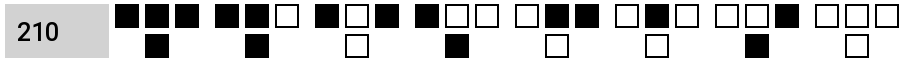
\includegraphics[width=\textwidth]{img/eca1.png}
		\caption{ECA 210}
		\label{img:eca1}
	\end{figure}
	
	El resultado de dicha regla se muestra en la figura \ref{img:eca2}. Se utiliza una segunda dimensión para representar el historial de la regla, aunque el comportamiento afecta únicamente la dimensión original.
	
	\begin{figure}[H]
		\centering
		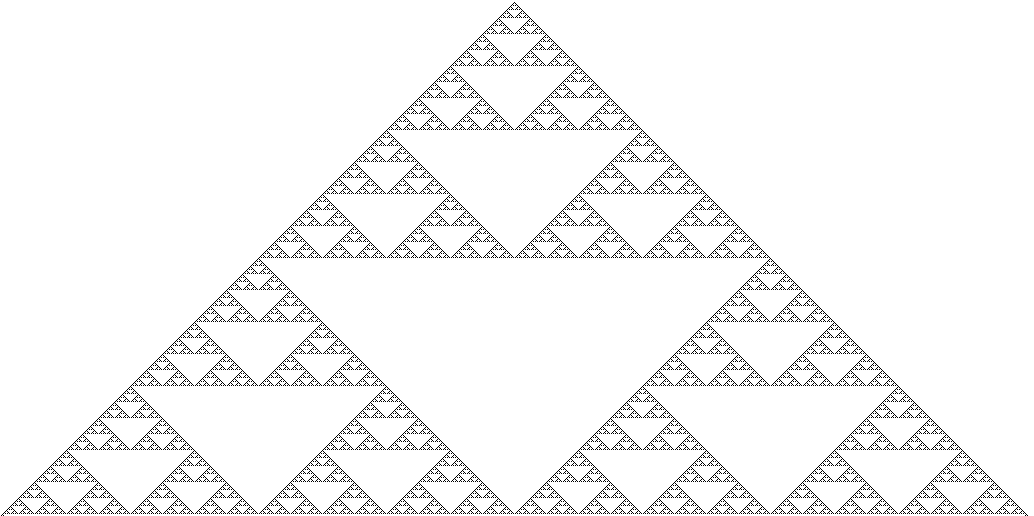
\includegraphics[width=\textwidth]{img/eca2.png}
		\caption{Evolución del ECA 210}
		\label{img:eca2}
	\end{figure}
	
	\subsection{Regla 30}
	
	La regla 30 equivale a $00011110_2$ en binario. Dada una única célula con valor 1, esta se expande en ambas direcciones con cada iteración, como se muestra en las figuras \ref{img:r30_1} y \ref{img:r30_2}, que ilustran las primeras 23 y 900 generaciones, respectivamente.
	
	Como se observa en la figura \ref{img:r30_2}, existe un pequeño patrón repetitivo que crece de forma diagonal en el lado izquierdo del historial. Sin embargo, en el lado derecho, el comportamiento no parece tener estabilidad ni un patrón discernible. Si almacenamos el historial de los valores de la célula inicial, se obtiene una secuencia pseudoaleatoria.
	
	Aunque no es posible predecir directamente si el siguiente estado será 0 o 1, es posible calcularlo realizando todas las generaciones previas.
	
	\begin{figure}[H]
		\centering
		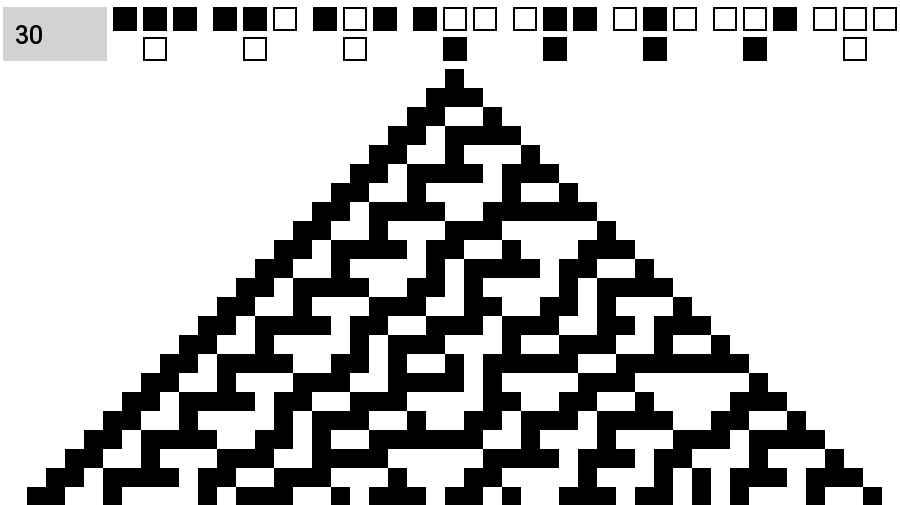
\includegraphics[width=\textwidth]{img/r30_1.png}
		\caption{Primeras 23 generaciones de la regla 30}
		\label{img:r30_1}
	\end{figure}
	
	\begin{figure}[H]
		\centering
		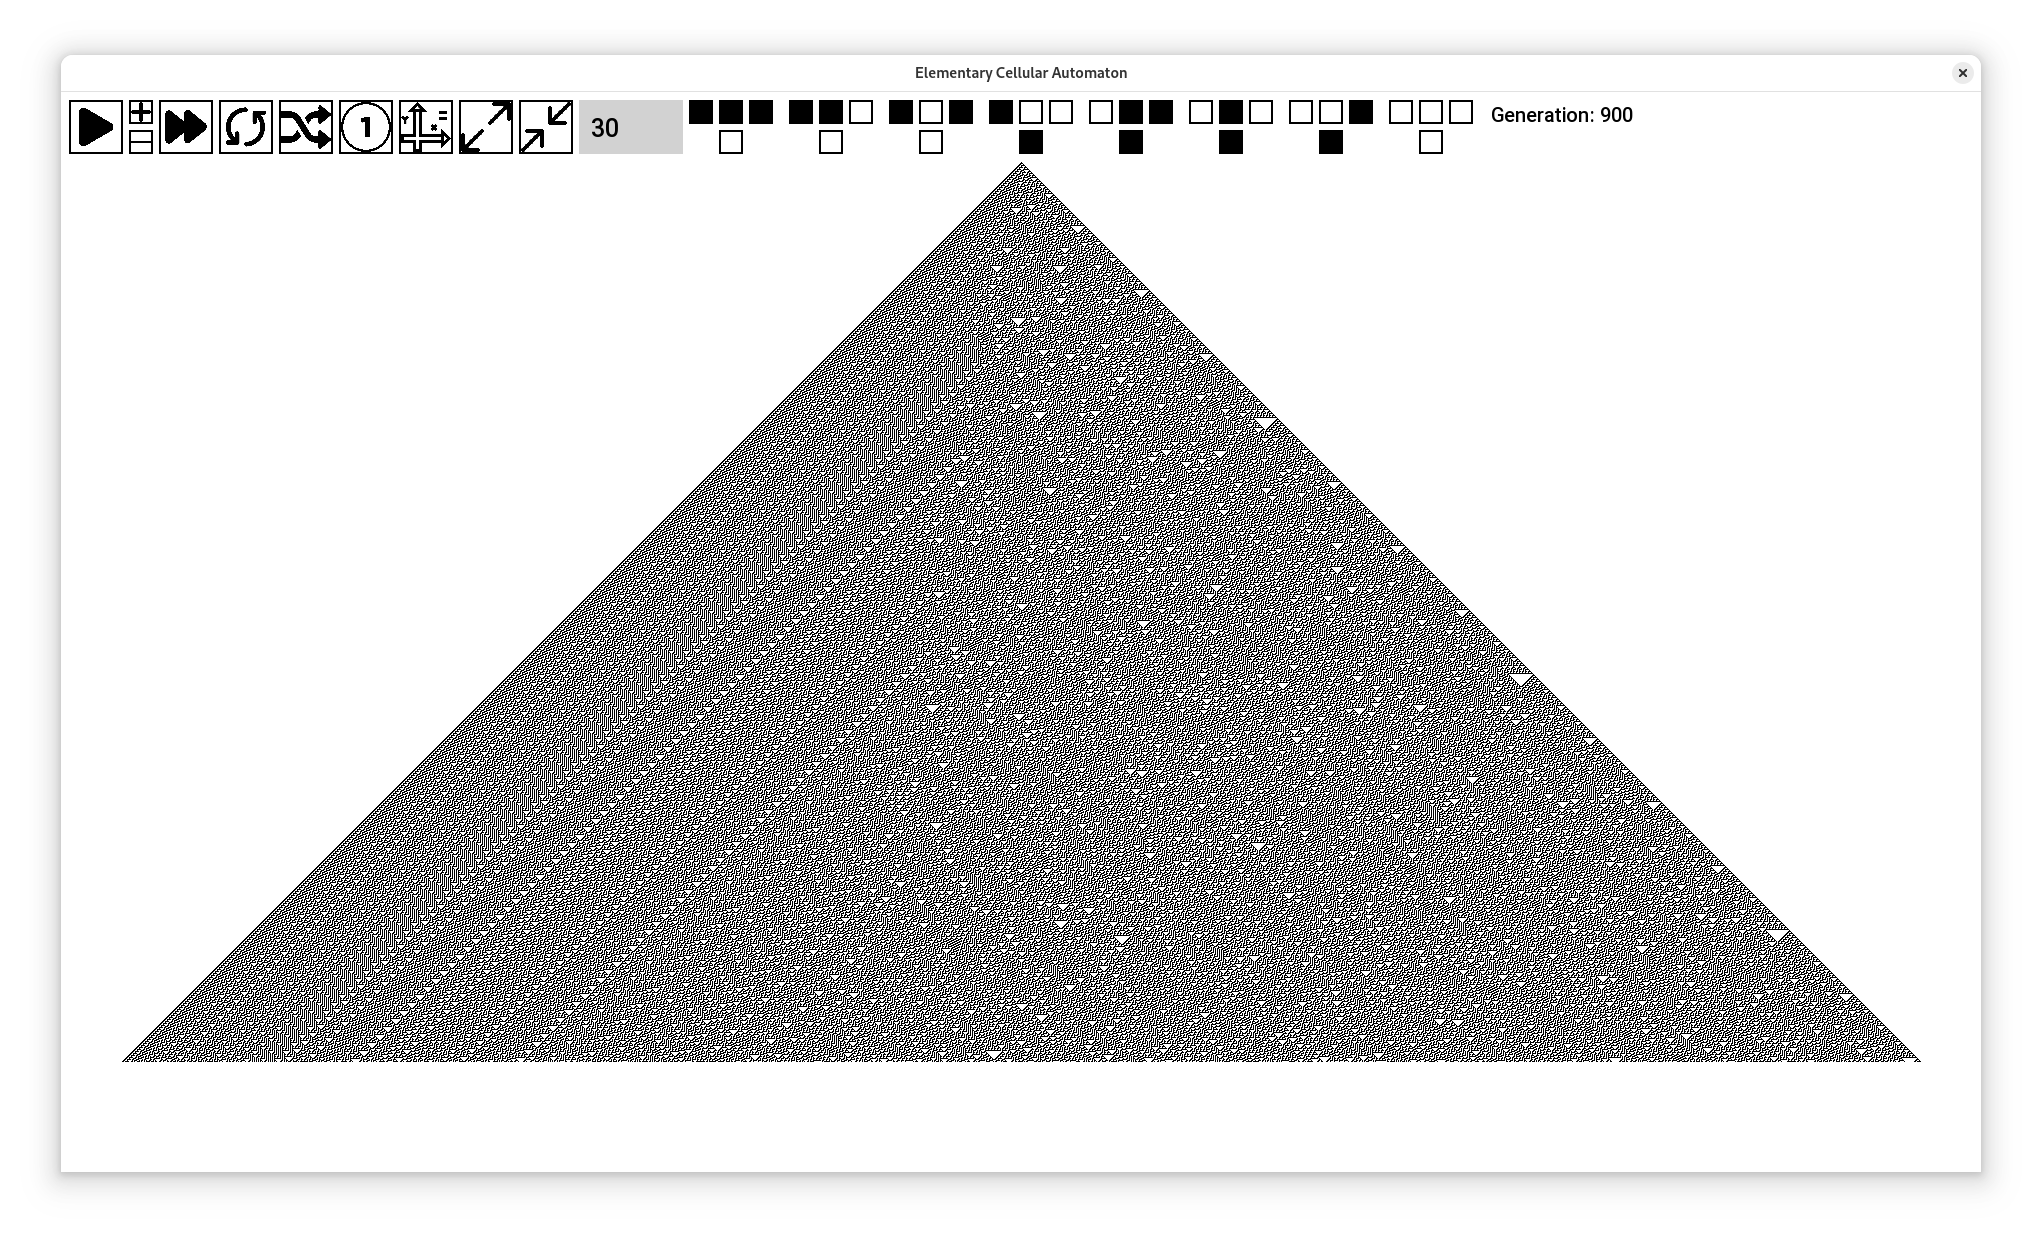
\includegraphics[width=\textwidth]{img/r30_2.png}
		\caption{Primeras 900 generaciones de la regla 30}
		\label{img:r30_2}
	\end{figure}
	
	\section{Metodología}
	
	El objetivo es encontrar un patrón en la columna principal. El primer análisis consiste en dividir el vector en todos los factores primos y medir el numero el numero de veces que la célula adquiere el valor el valor de 1.
	
	\subsection{Generación de datos}
	
	Se diseñó un programa en C++ con el objetivo de generar el mayor número de generaciones posibles. Cada generación es una secuencia de valores booleanos, que puede representarse como una cadena de valores binarios para ser almacenada como una secuencia de bytes en archivos de tipo binario.
	
	Cada generación se guarda en un archivo independiente, lo que permite acceder a ellas de forma individual. Esto asegura que, dada una generación $n$, sea posible calcular la generación $n+1$ sin necesidad de almacenar las $n-1$ generaciones anteriores.
	
	Debido a las limitaciones de visualización en el equipo de cómputo, se implementó una función que comprime todas las generaciones almacenadas en un único archivo.
	
	El número de operaciones depende del tamaño del vector, y dado que cada nueva generación aumenta en dos unidades y tiene una longitud impar, se puede utilizar la fórmula de la suma de Gauss para números impares:
	
	\begin{equation*}
		\sum_{i = 1}^{n} 2i - 1 = n^2
	\end{equation*}
	
	Para calcular el tiempo y el almacenamiento requeridos, se realizó una prueba inicial con un lote de 100,000 datos. A partir de los resultados, se estimaron los recursos necesarios para almacenar 2,500,000 datos en un disco duro externo.
	
	\begin{center}
		\begin{tabular}{|c|c|c|}
			\hline
			& \textbf{Valor calculado para} & \textbf{Valor aproximado para} \\
			& \textbf{100,000} & \textbf{2,500,000} \\
			\hline
			\textbf{Tiempo} & 32 minutos & $\approx$ 20,000 minutos $\approx$ 2 semanas \\
			\hline
			\textbf{Espacio} & 1.3 GB & $\approx$ 820 GB \\
			\hline
		\end{tabular}
	\end{center}
	
	\subsection{Extracción de características}
	
	Se diseña una función que itera todas las generaciones actualmente cargadas y extrae el valor de la columna principal, es decir, el valor en la posición $n$. Este paso se realiza con todas las generaciones hasta almacenar un vector de valores booleanos, que nuevamente se reescribe en un archivo de tipo binario.
	
	Ademas, se generan los primeros $m$ números primos menores a 1,250,000 para no tener que generarlos en tiempo real.
	
	\subsection{Segmentación}
	
	
	\clearpage
	\addcontentsline{toc}{section}{Referencias}
	\begin{thebibliography}{99}
		\bibitem{}
		
	
		
	\end{thebibliography}
	
\end{document}
